% Created by tikzDevice version 0.10.1 on 2016-03-21 19:09:18
% !TEX encoding = UTF-8 Unicode
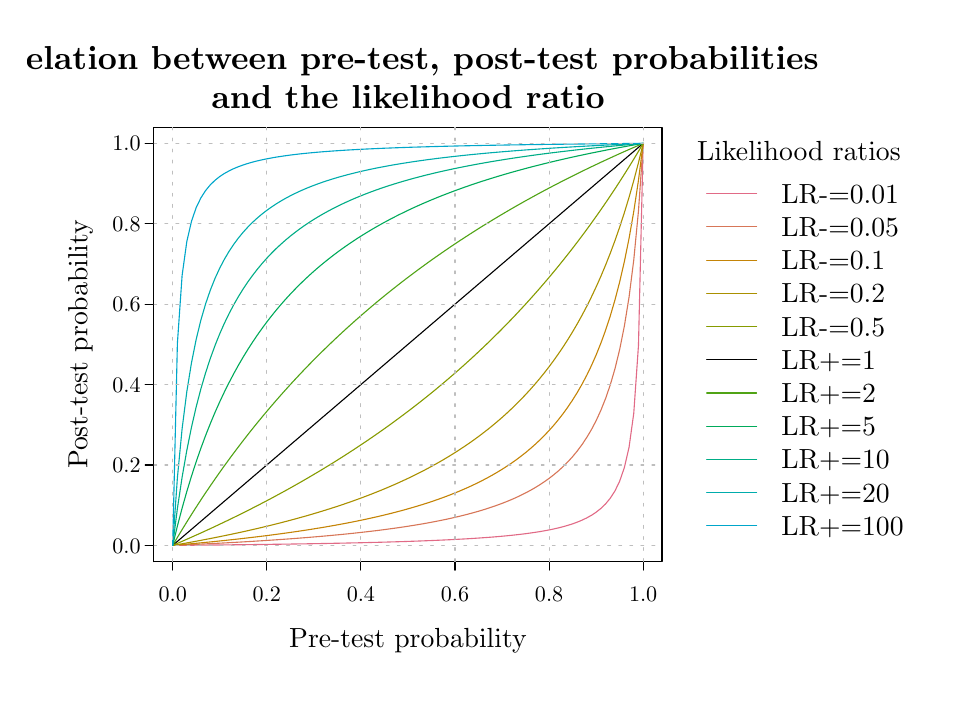
\begin{tikzpicture}[x=1pt,y=1pt]
\definecolor{fillColor}{RGB}{255,255,255}
\path[use as bounding box,fill=fillColor,fill opacity=0.00] (0,0) rectangle (325.21,238.49);
\begin{scope}
\path[clip] ( 45.60, 45.60) rectangle (229.21,202.49);
\definecolor{drawColor}{RGB}{0,0,0}

\path[draw=drawColor,line width= 0.4pt,line join=round,line cap=round] ( 52.40, 51.41) --
	( 54.10, 52.86) --
	( 55.80, 54.32) --
	( 57.50, 55.77) --
	( 59.20, 57.22) --
	( 60.90, 58.67) --
	( 62.60, 60.13) --
	( 64.30, 61.58) --
	( 66.00, 63.03) --
	( 67.70, 64.49) --
	( 69.40, 65.94) --
	( 71.10, 67.39) --
	( 72.80, 68.84) --
	( 74.50, 70.30) --
	( 76.20, 71.75) --
	( 77.90, 73.20) --
	( 79.60, 74.65) --
	( 81.30, 76.11) --
	( 83.00, 77.56) --
	( 84.70, 79.01) --
	( 86.40, 80.46) --
	( 88.10, 81.92) --
	( 89.80, 83.37) --
	( 91.50, 84.82) --
	( 93.20, 86.28) --
	( 94.90, 87.73) --
	( 96.60, 89.18) --
	( 98.30, 90.63) --
	(100.00, 92.09) --
	(101.70, 93.54) --
	(103.40, 94.99) --
	(105.10, 96.44) --
	(106.80, 97.90) --
	(108.51, 99.35) --
	(110.21,100.80) --
	(111.91,102.26) --
	(113.61,103.71) --
	(115.31,105.16) --
	(117.01,106.61) --
	(118.71,108.07) --
	(120.41,109.52) --
	(122.11,110.97) --
	(123.81,112.42) --
	(125.51,113.88) --
	(127.21,115.33) --
	(128.91,116.78) --
	(130.61,118.23) --
	(132.31,119.69) --
	(134.01,121.14) --
	(135.71,122.59) --
	(137.41,124.05) --
	(139.11,125.50) --
	(140.81,126.95) --
	(142.51,128.40) --
	(144.21,129.86) --
	(145.91,131.31) --
	(147.61,132.76) --
	(149.31,134.21) --
	(151.01,135.67) --
	(152.71,137.12) --
	(154.41,138.57) --
	(156.11,140.03) --
	(157.81,141.48) --
	(159.51,142.93) --
	(161.21,144.38) --
	(162.91,145.84) --
	(164.61,147.29) --
	(166.31,148.74) --
	(168.01,150.19) --
	(169.71,151.65) --
	(171.41,153.10) --
	(173.11,154.55) --
	(174.81,156.00) --
	(176.51,157.46) --
	(178.21,158.91) --
	(179.91,160.36) --
	(181.61,161.82) --
	(183.31,163.27) --
	(185.01,164.72) --
	(186.71,166.17) --
	(188.41,167.63) --
	(190.11,169.08) --
	(191.81,170.53) --
	(193.51,171.98) --
	(195.21,173.44) --
	(196.91,174.89) --
	(198.61,176.34) --
	(200.31,177.80) --
	(202.01,179.25) --
	(203.71,180.70) --
	(205.41,182.15) --
	(207.11,183.61) --
	(208.81,185.06) --
	(210.51,186.51) --
	(212.21,187.96) --
	(213.91,189.42) --
	(215.61,190.87) --
	(217.31,192.32) --
	(219.01,193.77) --
	(220.71,195.23) --
	(222.41,196.68);
\end{scope}
\begin{scope}
\path[clip] (  0.00,  0.00) rectangle (325.21,238.49);
\definecolor{drawColor}{RGB}{0,0,0}

\path[draw=drawColor,line width= 0.4pt,line join=round,line cap=round] ( 52.40, 45.60) -- (222.41, 45.60);

\path[draw=drawColor,line width= 0.4pt,line join=round,line cap=round] ( 52.40, 45.60) -- ( 52.40, 42.46);

\path[draw=drawColor,line width= 0.4pt,line join=round,line cap=round] ( 86.40, 45.60) -- ( 86.40, 42.46);

\path[draw=drawColor,line width= 0.4pt,line join=round,line cap=round] (120.41, 45.60) -- (120.41, 42.46);

\path[draw=drawColor,line width= 0.4pt,line join=round,line cap=round] (154.41, 45.60) -- (154.41, 42.46);

\path[draw=drawColor,line width= 0.4pt,line join=round,line cap=round] (188.41, 45.60) -- (188.41, 42.46);

\path[draw=drawColor,line width= 0.4pt,line join=round,line cap=round] (222.41, 45.60) -- (222.41, 42.46);

\node[text=drawColor,anchor=base,inner sep=0pt, outer sep=0pt, scale=  0.80] at ( 52.40, 31.20) {0.0};

\node[text=drawColor,anchor=base,inner sep=0pt, outer sep=0pt, scale=  0.80] at ( 86.40, 31.20) {0.2};

\node[text=drawColor,anchor=base,inner sep=0pt, outer sep=0pt, scale=  0.80] at (120.41, 31.20) {0.4};

\node[text=drawColor,anchor=base,inner sep=0pt, outer sep=0pt, scale=  0.80] at (154.41, 31.20) {0.6};

\node[text=drawColor,anchor=base,inner sep=0pt, outer sep=0pt, scale=  0.80] at (188.41, 31.20) {0.8};

\node[text=drawColor,anchor=base,inner sep=0pt, outer sep=0pt, scale=  0.80] at (222.41, 31.20) {1.0};

\path[draw=drawColor,line width= 0.4pt,line join=round,line cap=round] ( 45.60, 51.41) -- ( 45.60,196.68);

\path[draw=drawColor,line width= 0.4pt,line join=round,line cap=round] ( 45.60, 51.41) -- ( 42.46, 51.41);

\path[draw=drawColor,line width= 0.4pt,line join=round,line cap=round] ( 45.60, 80.46) -- ( 42.46, 80.46);

\path[draw=drawColor,line width= 0.4pt,line join=round,line cap=round] ( 45.60,109.52) -- ( 42.46,109.52);

\path[draw=drawColor,line width= 0.4pt,line join=round,line cap=round] ( 45.60,138.57) -- ( 42.46,138.57);

\path[draw=drawColor,line width= 0.4pt,line join=round,line cap=round] ( 45.60,167.63) -- ( 42.46,167.63);

\path[draw=drawColor,line width= 0.4pt,line join=round,line cap=round] ( 45.60,196.68) -- ( 42.46,196.68);

\node[text=drawColor,anchor=base east,inner sep=0pt, outer sep=0pt, scale=  0.80] at ( 40.80, 48.66) {0.0};

\node[text=drawColor,anchor=base east,inner sep=0pt, outer sep=0pt, scale=  0.80] at ( 40.80, 77.71) {0.2};

\node[text=drawColor,anchor=base east,inner sep=0pt, outer sep=0pt, scale=  0.80] at ( 40.80,106.76) {0.4};

\node[text=drawColor,anchor=base east,inner sep=0pt, outer sep=0pt, scale=  0.80] at ( 40.80,135.82) {0.6};

\node[text=drawColor,anchor=base east,inner sep=0pt, outer sep=0pt, scale=  0.80] at ( 40.80,164.87) {0.8};

\node[text=drawColor,anchor=base east,inner sep=0pt, outer sep=0pt, scale=  0.80] at ( 40.80,193.93) {1.0};

\path[draw=drawColor,line width= 0.4pt,line join=round,line cap=round] ( 45.60, 45.60) --
	(229.21, 45.60) --
	(229.21,202.49) --
	( 45.60,202.49) --
	( 45.60, 45.60);
\end{scope}
\begin{scope}
\path[clip] (  0.00,  0.00) rectangle (325.21,238.49);
\definecolor{drawColor}{RGB}{0,0,0}

\node[text=drawColor,anchor=base,inner sep=0pt, outer sep=0pt, scale=  1.20] at (137.41,223.55) {\bfseries Relation between pre-test, post-test probabilities};

\node[text=drawColor,anchor=base,inner sep=0pt, outer sep=0pt, scale=  1.20] at (137.41,209.15) {\bfseries  and the likelihood ratio};

\node[text=drawColor,anchor=base,inner sep=0pt, outer sep=0pt, scale=  1.00] at (137.41, 14.40) {Pre-test probability};

\node[text=drawColor,rotate= 90.00,anchor=base,inner sep=0pt, outer sep=0pt, scale=  1.00] at ( 21.60,124.05) {Post-test probability};
\end{scope}
\begin{scope}
\path[clip] ( 45.60, 45.60) rectangle (229.21,202.49);
\definecolor{drawColor}{RGB}{225,106,134}

\path[draw=drawColor,line width= 0.4pt,line join=round,line cap=round] ( 52.40, 51.41) --
	( 54.10, 51.43) --
	( 55.80, 51.44) --
	( 57.50, 51.46) --
	( 59.20, 51.47) --
	( 60.90, 51.49) --
	( 62.60, 51.50) --
	( 64.30, 51.52) --
	( 66.00, 51.54) --
	( 67.70, 51.55) --
	( 69.40, 51.57) --
	( 71.10, 51.59) --
	( 72.80, 51.61) --
	( 74.50, 51.63) --
	( 76.20, 51.65) --
	( 77.90, 51.67) --
	( 79.60, 51.69) --
	( 81.30, 51.71) --
	( 83.00, 51.73) --
	( 84.70, 51.75) --
	( 86.40, 51.77) --
	( 88.10, 51.80) --
	( 89.80, 51.82) --
	( 91.50, 51.84) --
	( 93.20, 51.87) --
	( 94.90, 51.89) --
	( 96.60, 51.92) --
	( 98.30, 51.95) --
	(100.00, 51.97) --
	(101.70, 52.00) --
	(103.40, 52.03) --
	(105.10, 52.06) --
	(106.80, 52.09) --
	(108.51, 52.12) --
	(110.21, 52.16) --
	(111.91, 52.19) --
	(113.61, 52.22) --
	(115.31, 52.26) --
	(117.01, 52.30) --
	(118.71, 52.33) --
	(120.41, 52.37) --
	(122.11, 52.41) --
	(123.81, 52.46) --
	(125.51, 52.50) --
	(127.21, 52.54) --
	(128.91, 52.59) --
	(130.61, 52.64) --
	(132.31, 52.69) --
	(134.01, 52.74) --
	(135.71, 52.79) --
	(137.41, 52.85) --
	(139.11, 52.91) --
	(140.81, 52.97) --
	(142.51, 53.03) --
	(144.21, 53.10) --
	(145.91, 53.16) --
	(147.61, 53.24) --
	(149.31, 53.31) --
	(151.01, 53.39) --
	(152.71, 53.47) --
	(154.41, 53.56) --
	(156.11, 53.65) --
	(157.81, 53.74) --
	(159.51, 53.84) --
	(161.21, 53.95) --
	(162.91, 54.06) --
	(164.61, 54.18) --
	(166.31, 54.30) --
	(168.01, 54.43) --
	(169.71, 54.57) --
	(171.41, 54.72) --
	(173.11, 54.88) --
	(174.81, 55.05) --
	(176.51, 55.24) --
	(178.21, 55.43) --
	(179.91, 55.64) --
	(181.61, 55.87) --
	(183.31, 56.12) --
	(185.01, 56.38) --
	(186.71, 56.68) --
	(188.41, 57.00) --
	(190.11, 57.35) --
	(191.81, 57.74) --
	(193.51, 58.17) --
	(195.21, 58.66) --
	(196.91, 59.20) --
	(198.61, 59.82) --
	(200.31, 60.52) --
	(202.01, 61.34) --
	(203.71, 62.28) --
	(205.41, 63.41) --
	(207.11, 64.75) --
	(208.81, 66.39) --
	(210.51, 68.45) --
	(212.21, 71.09) --
	(213.91, 74.61) --
	(215.61, 79.53) --
	(217.31, 86.90) --
	(219.01, 99.18) --
	(220.71,123.68) --
	(222.41,196.68);
\definecolor{drawColor}{RGB}{215,118,88}

\path[draw=drawColor,line width= 0.4pt,line join=round,line cap=round] ( 52.40, 51.41) --
	( 54.10, 51.48) --
	( 55.80, 51.56) --
	( 57.50, 51.64) --
	( 59.20, 51.71) --
	( 60.90, 51.79) --
	( 62.60, 51.87) --
	( 64.30, 51.96) --
	( 66.00, 52.04) --
	( 67.70, 52.13) --
	( 69.40, 52.21) --
	( 71.10, 52.30) --
	( 72.80, 52.39) --
	( 74.50, 52.49) --
	( 76.20, 52.58) --
	( 77.90, 52.68) --
	( 79.60, 52.78) --
	( 81.30, 52.88) --
	( 83.00, 52.99) --
	( 84.70, 53.09) --
	( 86.40, 53.20) --
	( 88.10, 53.32) --
	( 89.80, 53.43) --
	( 91.50, 53.55) --
	( 93.20, 53.67) --
	( 94.90, 53.79) --
	( 96.60, 53.92) --
	( 98.30, 54.05) --
	(100.00, 54.18) --
	(101.70, 54.32) --
	(103.40, 54.46) --
	(105.10, 54.60) --
	(106.80, 54.75) --
	(108.51, 54.90) --
	(110.21, 55.06) --
	(111.91, 55.22) --
	(113.61, 55.38) --
	(115.31, 55.55) --
	(117.01, 55.73) --
	(118.71, 55.91) --
	(120.41, 56.10) --
	(122.11, 56.29) --
	(123.81, 56.49) --
	(125.51, 56.69) --
	(127.21, 56.90) --
	(128.91, 57.12) --
	(130.61, 57.35) --
	(132.31, 57.58) --
	(134.01, 57.82) --
	(135.71, 58.07) --
	(137.41, 58.33) --
	(139.11, 58.60) --
	(140.81, 58.88) --
	(142.51, 59.16) --
	(144.21, 59.46) --
	(145.91, 59.78) --
	(147.61, 60.10) --
	(149.31, 60.44) --
	(151.01, 60.79) --
	(152.71, 61.16) --
	(154.41, 61.55) --
	(156.11, 61.95) --
	(157.81, 62.37) --
	(159.51, 62.81) --
	(161.21, 63.27) --
	(162.91, 63.75) --
	(164.61, 64.26) --
	(166.31, 64.80) --
	(168.01, 65.36) --
	(169.71, 65.96) --
	(171.41, 66.59) --
	(173.11, 67.25) --
	(174.81, 67.96) --
	(176.51, 68.71) --
	(178.21, 69.51) --
	(179.91, 70.36) --
	(181.61, 71.27) --
	(183.31, 72.24) --
	(185.01, 73.29) --
	(186.71, 74.41) --
	(188.41, 75.62) --
	(190.11, 76.94) --
	(191.81, 78.36) --
	(193.51, 79.92) --
	(195.21, 81.62) --
	(196.91, 83.48) --
	(198.61, 85.55) --
	(200.31, 87.83) --
	(202.01, 90.39) --
	(203.71, 93.25) --
	(205.41, 96.49) --
	(207.11,100.19) --
	(208.81,104.45) --
	(210.51,109.39) --
	(212.21,115.22) --
	(213.91,122.18) --
	(215.61,130.65) --
	(217.31,141.16) --
	(219.01,154.57) --
	(220.71,172.27) --
	(222.41,196.68);
\definecolor{drawColor}{RGB}{196,132,7}

\path[draw=drawColor,line width= 0.4pt,line join=round,line cap=round] ( 52.40, 51.41) --
	( 54.10, 51.56) --
	( 55.80, 51.71) --
	( 57.50, 51.86) --
	( 59.20, 52.01) --
	( 60.90, 52.17) --
	( 62.60, 52.33) --
	( 64.30, 52.50) --
	( 66.00, 52.66) --
	( 67.70, 52.83) --
	( 69.40, 53.01) --
	( 71.10, 53.18) --
	( 72.80, 53.37) --
	( 74.50, 53.55) --
	( 76.20, 53.74) --
	( 77.90, 53.93) --
	( 79.60, 54.13) --
	( 81.30, 54.33) --
	( 83.00, 54.53) --
	( 84.70, 54.74) --
	( 86.40, 54.95) --
	( 88.10, 55.17) --
	( 89.80, 55.40) --
	( 91.50, 55.62) --
	( 93.20, 55.86) --
	( 94.90, 56.10) --
	( 96.60, 56.34) --
	( 98.30, 56.59) --
	(100.00, 56.85) --
	(101.70, 57.11) --
	(103.40, 57.38) --
	(105.10, 57.66) --
	(106.80, 57.94) --
	(108.51, 58.23) --
	(110.21, 58.53) --
	(111.91, 58.83) --
	(113.61, 59.15) --
	(115.31, 59.47) --
	(117.01, 59.80) --
	(118.71, 60.14) --
	(120.41, 60.49) --
	(122.11, 60.85) --
	(123.81, 61.22) --
	(125.51, 61.60) --
	(127.21, 61.99) --
	(128.91, 62.40) --
	(130.61, 62.81) --
	(132.31, 63.24) --
	(134.01, 63.69) --
	(135.71, 64.14) --
	(137.41, 64.62) --
	(139.11, 65.11) --
	(140.81, 65.61) --
	(142.51, 66.13) --
	(144.21, 66.67) --
	(145.91, 67.23) --
	(147.61, 67.81) --
	(149.31, 68.41) --
	(151.01, 69.04) --
	(152.71, 69.69) --
	(154.41, 70.36) --
	(156.11, 71.06) --
	(157.81, 71.79) --
	(159.51, 72.55) --
	(161.21, 73.34) --
	(162.91, 74.16) --
	(164.61, 75.03) --
	(166.31, 75.93) --
	(168.01, 76.87) --
	(169.71, 77.86) --
	(171.41, 78.89) --
	(173.11, 79.98) --
	(174.81, 81.12) --
	(176.51, 82.33) --
	(178.21, 83.60) --
	(179.91, 84.93) --
	(181.61, 86.35) --
	(183.31, 87.85) --
	(185.01, 89.43) --
	(186.71, 91.12) --
	(188.41, 92.92) --
	(190.11, 94.83) --
	(191.81, 96.88) --
	(193.51, 99.07) --
	(195.21,101.42) --
	(196.91,103.96) --
	(198.61,106.69) --
	(200.31,109.65) --
	(202.01,112.87) --
	(203.71,116.38) --
	(205.41,120.22) --
	(207.11,124.45) --
	(208.81,129.11) --
	(210.51,134.29) --
	(212.21,140.08) --
	(213.91,146.59) --
	(215.61,153.95) --
	(217.31,162.36) --
	(219.01,172.06) --
	(220.71,183.35) --
	(222.41,196.68);
\definecolor{drawColor}{RGB}{170,144,0}

\path[draw=drawColor,line width= 0.4pt,line join=round,line cap=round] ( 52.40, 51.41) --
	( 54.10, 51.70) --
	( 55.80, 52.00) --
	( 57.50, 52.30) --
	( 59.20, 52.61) --
	( 60.90, 52.92) --
	( 62.60, 53.24) --
	( 64.30, 53.57) --
	( 66.00, 53.89) --
	( 67.70, 54.23) --
	( 69.40, 54.57) --
	( 71.10, 54.92) --
	( 72.80, 55.27) --
	( 74.50, 55.63) --
	( 76.20, 55.99) --
	( 77.90, 56.36) --
	( 79.60, 56.74) --
	( 81.30, 57.13) --
	( 83.00, 57.52) --
	( 84.70, 57.92) --
	( 86.40, 58.33) --
	( 88.10, 58.74) --
	( 89.80, 59.17) --
	( 91.50, 59.60) --
	( 93.20, 60.04) --
	( 94.90, 60.49) --
	( 96.60, 60.95) --
	( 98.30, 61.42) --
	(100.00, 61.89) --
	(101.70, 62.38) --
	(103.40, 62.88) --
	(105.10, 63.39) --
	(106.80, 63.91) --
	(108.51, 64.44) --
	(110.21, 64.98) --
	(111.91, 65.53) --
	(113.61, 66.10) --
	(115.31, 66.68) --
	(117.01, 67.27) --
	(118.71, 67.88) --
	(120.41, 68.50) --
	(122.11, 69.14) --
	(123.81, 69.79) --
	(125.51, 70.46) --
	(127.21, 71.14) --
	(128.91, 71.84) --
	(130.61, 72.56) --
	(132.31, 73.29) --
	(134.01, 74.05) --
	(135.71, 74.83) --
	(137.41, 75.62) --
	(139.11, 76.44) --
	(140.81, 77.28) --
	(142.51, 78.14) --
	(144.21, 79.03) --
	(145.91, 79.95) --
	(147.61, 80.89) --
	(149.31, 81.85) --
	(151.01, 82.85) --
	(152.71, 83.88) --
	(154.41, 84.93) --
	(156.11, 86.03) --
	(157.81, 87.15) --
	(159.51, 88.31) --
	(161.21, 89.51) --
	(162.91, 90.75) --
	(164.61, 92.04) --
	(166.31, 93.36) --
	(168.01, 94.74) --
	(169.71, 96.16) --
	(171.41, 97.63) --
	(173.11, 99.16) --
	(174.81,100.75) --
	(176.51,102.39) --
	(178.21,104.11) --
	(179.91,105.89) --
	(181.61,107.74) --
	(183.31,109.67) --
	(185.01,111.68) --
	(186.71,113.78) --
	(188.41,115.97) --
	(190.11,118.27) --
	(191.81,120.67) --
	(193.51,123.18) --
	(195.21,125.82) --
	(196.91,128.59) --
	(198.61,131.50) --
	(200.31,134.56) --
	(202.01,137.79) --
	(203.71,141.20) --
	(205.41,144.80) --
	(207.11,148.61) --
	(208.81,152.66) --
	(210.51,156.96) --
	(212.21,161.53) --
	(213.91,166.42) --
	(215.61,171.63) --
	(217.31,177.22) --
	(219.01,183.23) --
	(220.71,189.70) --
	(222.41,196.68);
\definecolor{drawColor}{RGB}{134,155,0}

\path[draw=drawColor,line width= 0.4pt,line join=round,line cap=round] ( 52.40, 51.41) --
	( 54.10, 52.14) --
	( 55.80, 52.88) --
	( 57.50, 53.62) --
	( 59.20, 54.38) --
	( 60.90, 55.14) --
	( 62.60, 55.90) --
	( 64.30, 56.68) --
	( 66.00, 57.46) --
	( 67.70, 58.26) --
	( 69.40, 59.06) --
	( 71.10, 59.87) --
	( 72.80, 60.68) --
	( 74.50, 61.51) --
	( 76.20, 62.35) --
	( 77.90, 63.19) --
	( 79.60, 64.04) --
	( 81.30, 64.91) --
	( 83.00, 65.78) --
	( 84.70, 66.66) --
	( 86.40, 67.55) --
	( 88.10, 68.45) --
	( 89.80, 69.37) --
	( 91.50, 70.29) --
	( 93.20, 71.22) --
	( 94.90, 72.16) --
	( 96.60, 73.12) --
	( 98.30, 74.08) --
	(100.00, 75.06) --
	(101.70, 76.05) --
	(103.40, 77.05) --
	(105.10, 78.06) --
	(106.80, 79.08) --
	(108.51, 80.12) --
	(110.21, 81.16) --
	(111.91, 82.23) --
	(113.61, 83.30) --
	(115.31, 84.39) --
	(117.01, 85.49) --
	(118.71, 86.60) --
	(120.41, 87.73) --
	(122.11, 88.87) --
	(123.81, 90.03) --
	(125.51, 91.20) --
	(127.21, 92.38) --
	(128.91, 93.59) --
	(130.61, 94.80) --
	(132.31, 96.04) --
	(134.01, 97.29) --
	(135.71, 98.55) --
	(137.41, 99.83) --
	(139.11,101.13) --
	(140.81,102.45) --
	(142.51,103.79) --
	(144.21,105.14) --
	(145.91,106.51) --
	(147.61,107.90) --
	(149.31,109.32) --
	(151.01,110.75) --
	(152.71,112.20) --
	(154.41,113.67) --
	(156.11,115.16) --
	(157.81,116.68) --
	(159.51,118.21) --
	(161.21,119.77) --
	(162.91,121.36) --
	(164.61,122.96) --
	(166.31,124.59) --
	(168.01,126.25) --
	(169.71,127.93) --
	(171.41,129.63) --
	(173.11,131.37) --
	(174.81,133.12) --
	(176.51,134.91) --
	(178.21,136.73) --
	(179.91,138.57) --
	(181.61,140.45) --
	(183.31,142.35) --
	(185.01,144.29) --
	(186.71,146.26) --
	(188.41,148.26) --
	(190.11,150.29) --
	(191.81,152.36) --
	(193.51,154.47) --
	(195.21,156.61) --
	(196.91,158.78) --
	(198.61,161.00) --
	(200.31,163.26) --
	(202.01,165.55) --
	(203.71,167.89) --
	(205.41,170.27) --
	(207.11,172.69) --
	(208.81,175.16) --
	(210.51,177.67) --
	(212.21,180.23) --
	(213.91,182.85) --
	(215.61,185.51) --
	(217.31,188.22) --
	(219.01,190.98) --
	(220.71,193.80) --
	(222.41,196.68);
\definecolor{drawColor}{RGB}{80,163,21}

\path[draw=drawColor,line width= 0.4pt,line join=round,line cap=round] ( 52.40, 51.41) --
	( 54.10, 54.29) --
	( 55.80, 57.11) --
	( 57.50, 59.87) --
	( 59.20, 62.59) --
	( 60.90, 65.25) --
	( 62.60, 67.86) --
	( 64.30, 70.42) --
	( 66.00, 72.93) --
	( 67.70, 75.40) --
	( 69.40, 77.82) --
	( 71.10, 80.20) --
	( 72.80, 82.54) --
	( 74.50, 84.84) --
	( 76.20, 87.09) --
	( 77.90, 89.31) --
	( 79.60, 91.49) --
	( 81.30, 93.63) --
	( 83.00, 95.73) --
	( 84.70, 97.80) --
	( 86.40, 99.83) --
	( 88.10,101.83) --
	( 89.80,103.80) --
	( 91.50,105.74) --
	( 93.20,107.64) --
	( 94.90,109.52) --
	( 96.60,111.36) --
	( 98.30,113.18) --
	(100.00,114.97) --
	(101.70,116.73) --
	(103.40,118.46) --
	(105.10,120.16) --
	(106.80,121.84) --
	(108.51,123.50) --
	(110.21,125.13) --
	(111.91,126.74) --
	(113.61,128.32) --
	(115.31,129.88) --
	(117.01,131.41) --
	(118.71,132.93) --
	(120.41,134.42) --
	(122.11,135.89) --
	(123.81,137.34) --
	(125.51,138.78) --
	(127.21,140.19) --
	(128.91,141.58) --
	(130.61,142.95) --
	(132.31,144.30) --
	(134.01,145.64) --
	(135.71,146.96) --
	(137.41,148.26) --
	(139.11,149.54) --
	(140.81,150.81) --
	(142.51,152.05) --
	(144.21,153.29) --
	(145.91,154.51) --
	(147.61,155.71) --
	(149.31,156.89) --
	(151.01,158.06) --
	(152.71,159.22) --
	(154.41,160.36) --
	(156.11,161.49) --
	(157.81,162.60) --
	(159.51,163.70) --
	(161.21,164.79) --
	(162.91,165.87) --
	(164.61,166.93) --
	(166.31,167.97) --
	(168.01,169.01) --
	(169.71,170.03) --
	(171.41,171.04) --
	(173.11,172.04) --
	(174.81,173.03) --
	(176.51,174.01) --
	(178.21,174.97) --
	(179.91,175.93) --
	(181.61,176.87) --
	(183.31,177.80) --
	(185.01,178.73) --
	(186.71,179.64) --
	(188.41,180.54) --
	(190.11,181.43) --
	(191.81,182.31) --
	(193.51,183.19) --
	(195.21,184.05) --
	(196.91,184.90) --
	(198.61,185.75) --
	(200.31,186.58) --
	(202.01,187.41) --
	(203.71,188.23) --
	(205.41,189.03) --
	(207.11,189.84) --
	(208.81,190.63) --
	(210.51,191.41) --
	(212.21,192.19) --
	(213.91,192.96) --
	(215.61,193.72) --
	(217.31,194.47) --
	(219.01,195.21) --
	(220.71,195.95) --
	(222.41,196.68);
\definecolor{drawColor}{RGB}{0,170,90}

\path[draw=drawColor,line width= 0.4pt,line join=round,line cap=round] ( 52.40, 51.41) --
	( 54.10, 58.39) --
	( 55.80, 64.86) --
	( 57.50, 70.87) --
	( 59.20, 76.46) --
	( 60.90, 81.68) --
	( 62.60, 86.56) --
	( 64.30, 91.13) --
	( 66.00, 95.43) --
	( 67.70, 99.48) --
	( 69.40,103.29) --
	( 71.10,106.90) --
	( 72.80,110.30) --
	( 74.50,113.53) --
	( 76.20,116.60) --
	( 77.90,119.51) --
	( 79.60,122.27) --
	( 81.30,124.91) --
	( 83.00,127.42) --
	( 84.70,129.82) --
	( 86.40,132.12) --
	( 88.10,134.31) --
	( 89.80,136.41) --
	( 91.50,138.42) --
	( 93.20,140.35) --
	( 94.90,142.20) --
	( 96.60,143.98) --
	( 98.30,145.70) --
	(100.00,147.34) --
	(101.70,148.93) --
	(103.40,150.46) --
	(105.10,151.93) --
	(106.80,153.35) --
	(108.51,154.73) --
	(110.21,156.05) --
	(111.91,157.34) --
	(113.61,158.58) --
	(115.31,159.78) --
	(117.01,160.94) --
	(118.71,162.07) --
	(120.41,163.16) --
	(122.11,164.21) --
	(123.81,165.24) --
	(125.51,166.24) --
	(127.21,167.21) --
	(128.91,168.15) --
	(130.61,169.06) --
	(132.31,169.95) --
	(134.01,170.81) --
	(135.71,171.65) --
	(137.41,172.47) --
	(139.11,173.27) --
	(140.81,174.04) --
	(142.51,174.80) --
	(144.21,175.53) --
	(145.91,176.25) --
	(147.61,176.95) --
	(149.31,177.64) --
	(151.01,178.30) --
	(152.71,178.95) --
	(154.41,179.59) --
	(156.11,180.21) --
	(157.81,180.82) --
	(159.51,181.41) --
	(161.21,181.99) --
	(162.91,182.56) --
	(164.61,183.11) --
	(166.31,183.65) --
	(168.01,184.18) --
	(169.71,184.70) --
	(171.41,185.21) --
	(173.11,185.71) --
	(174.81,186.20) --
	(176.51,186.67) --
	(178.21,187.14) --
	(179.91,187.60) --
	(181.61,188.05) --
	(183.31,188.49) --
	(185.01,188.92) --
	(186.71,189.35) --
	(188.41,189.76) --
	(190.11,190.17) --
	(191.81,190.57) --
	(193.51,190.96) --
	(195.21,191.35) --
	(196.91,191.73) --
	(198.61,192.10) --
	(200.31,192.46) --
	(202.01,192.82) --
	(203.71,193.18) --
	(205.41,193.52) --
	(207.11,193.86) --
	(208.81,194.20) --
	(210.51,194.53) --
	(212.21,194.85) --
	(213.91,195.17) --
	(215.61,195.48) --
	(217.31,195.79) --
	(219.01,196.09) --
	(220.71,196.39) --
	(222.41,196.68);
\definecolor{drawColor}{RGB}{0,173,134}

\path[draw=drawColor,line width= 0.4pt,line join=round,line cap=round] ( 52.40, 51.41) --
	( 54.10, 64.74) --
	( 55.80, 76.03) --
	( 57.50, 85.73) --
	( 59.20, 94.14) --
	( 60.90,101.50) --
	( 62.60,108.01) --
	( 64.30,113.80) --
	( 66.00,118.98) --
	( 67.70,123.64) --
	( 69.40,127.87) --
	( 71.10,131.71) --
	( 72.80,135.22) --
	( 74.50,138.44) --
	( 76.20,141.40) --
	( 77.90,144.14) --
	( 79.60,146.67) --
	( 81.30,149.02) --
	( 83.00,151.21) --
	( 84.70,153.26) --
	( 86.40,155.17) --
	( 88.10,156.97) --
	( 89.80,158.66) --
	( 91.50,160.24) --
	( 93.20,161.74) --
	( 94.90,163.16) --
	( 96.60,164.49) --
	( 98.30,165.76) --
	(100.00,166.97) --
	(101.70,168.11) --
	(103.40,169.20) --
	(105.10,170.23) --
	(106.80,171.22) --
	(108.51,172.16) --
	(110.21,173.06) --
	(111.91,173.93) --
	(113.61,174.75) --
	(115.31,175.54) --
	(117.01,176.30) --
	(118.71,177.03) --
	(120.41,177.73) --
	(122.11,178.41) --
	(123.81,179.05) --
	(125.51,179.68) --
	(127.21,180.28) --
	(128.91,180.86) --
	(130.61,181.42) --
	(132.31,181.96) --
	(134.01,182.48) --
	(135.71,182.99) --
	(137.41,183.47) --
	(139.11,183.95) --
	(140.81,184.40) --
	(142.51,184.85) --
	(144.21,185.28) --
	(145.91,185.69) --
	(147.61,186.10) --
	(149.31,186.49) --
	(151.01,186.87) --
	(152.71,187.24) --
	(154.41,187.60) --
	(156.11,187.95) --
	(157.81,188.29) --
	(159.51,188.62) --
	(161.21,188.94) --
	(162.91,189.26) --
	(164.61,189.56) --
	(166.31,189.86) --
	(168.01,190.15) --
	(169.71,190.43) --
	(171.41,190.71) --
	(173.11,190.98) --
	(174.81,191.24) --
	(176.51,191.50) --
	(178.21,191.75) --
	(179.91,191.99) --
	(181.61,192.23) --
	(183.31,192.47) --
	(185.01,192.70) --
	(186.71,192.92) --
	(188.41,193.14) --
	(190.11,193.35) --
	(191.81,193.56) --
	(193.51,193.76) --
	(195.21,193.96) --
	(196.91,194.16) --
	(198.61,194.35) --
	(200.31,194.54) --
	(202.01,194.73) --
	(203.71,194.91) --
	(205.41,195.08) --
	(207.11,195.26) --
	(208.81,195.43) --
	(210.51,195.59) --
	(212.21,195.76) --
	(213.91,195.92) --
	(215.61,196.08) --
	(217.31,196.23) --
	(219.01,196.38) --
	(220.71,196.53) --
	(222.41,196.68);
\definecolor{drawColor}{RGB}{0,172,172}

\path[draw=drawColor,line width= 0.4pt,line join=round,line cap=round] ( 52.40, 51.41) --
	( 54.10, 75.83) --
	( 55.80, 93.52) --
	( 57.50,106.93) --
	( 59.20,117.44) --
	( 60.90,125.91) --
	( 62.60,132.87) --
	( 64.30,138.70) --
	( 66.00,143.65) --
	( 67.70,147.90) --
	( 69.40,151.60) --
	( 71.10,154.84) --
	( 72.80,157.71) --
	( 74.50,160.26) --
	( 76.20,162.55) --
	( 77.90,164.61) --
	( 79.60,166.48) --
	( 81.30,168.18) --
	( 83.00,169.73) --
	( 84.70,171.16) --
	( 86.40,172.47) --
	( 88.10,173.68) --
	( 89.80,174.81) --
	( 91.50,175.85) --
	( 93.20,176.82) --
	( 94.90,177.73) --
	( 96.60,178.58) --
	( 98.30,179.38) --
	(100.00,180.13) --
	(101.70,180.84) --
	(103.40,181.50) --
	(105.10,182.13) --
	(106.80,182.73) --
	(108.51,183.29) --
	(110.21,183.83) --
	(111.91,184.34) --
	(113.61,184.82) --
	(115.31,185.28) --
	(117.01,185.72) --
	(118.71,186.14) --
	(120.41,186.55) --
	(122.11,186.93) --
	(123.81,187.30) --
	(125.51,187.65) --
	(127.21,187.99) --
	(128.91,188.31) --
	(130.61,188.63) --
	(132.31,188.93) --
	(134.01,189.22) --
	(135.71,189.49) --
	(137.41,189.76) --
	(139.11,190.02) --
	(140.81,190.27) --
	(142.51,190.51) --
	(144.21,190.75) --
	(145.91,190.97) --
	(147.61,191.19) --
	(149.31,191.40) --
	(151.01,191.60) --
	(152.71,191.80) --
	(154.41,191.99) --
	(156.11,192.18) --
	(157.81,192.36) --
	(159.51,192.54) --
	(161.21,192.71) --
	(162.91,192.87) --
	(164.61,193.03) --
	(166.31,193.19) --
	(168.01,193.34) --
	(169.71,193.49) --
	(171.41,193.63) --
	(173.11,193.77) --
	(174.81,193.91) --
	(176.51,194.04) --
	(178.21,194.17) --
	(179.91,194.30) --
	(181.61,194.42) --
	(183.31,194.54) --
	(185.01,194.66) --
	(186.71,194.77) --
	(188.41,194.89) --
	(190.11,195.00) --
	(191.81,195.10) --
	(193.51,195.21) --
	(195.21,195.31) --
	(196.91,195.41) --
	(198.61,195.51) --
	(200.31,195.60) --
	(202.01,195.70) --
	(203.71,195.79) --
	(205.41,195.88) --
	(207.11,195.97) --
	(208.81,196.05) --
	(210.51,196.14) --
	(212.21,196.22) --
	(213.91,196.30) --
	(215.61,196.38) --
	(217.31,196.46) --
	(219.01,196.53) --
	(220.71,196.61) --
	(222.41,196.68);
\definecolor{drawColor}{RGB}{0,166,202}

\path[draw=drawColor,line width= 0.4pt,line join=round,line cap=round] ( 52.40, 51.41) --
	( 54.10,124.41) --
	( 55.80,148.91) --
	( 57.50,161.19) --
	( 59.20,168.56) --
	( 60.90,173.49) --
	( 62.60,177.00) --
	( 64.30,179.64) --
	( 66.00,181.70) --
	( 67.70,183.34) --
	( 69.40,184.69) --
	( 71.10,185.81) --
	( 72.80,186.75) --
	( 74.50,187.57) --
	( 76.20,188.27) --
	( 77.90,188.89) --
	( 79.60,189.43) --
	( 81.30,189.92) --
	( 83.00,190.35) --
	( 84.70,190.74) --
	( 86.40,191.09) --
	( 88.10,191.41) --
	( 89.80,191.71) --
	( 91.50,191.97) --
	( 93.20,192.22) --
	( 94.90,192.45) --
	( 96.60,192.66) --
	( 98.30,192.86) --
	(100.00,193.04) --
	(101.70,193.21) --
	(103.40,193.37) --
	(105.10,193.52) --
	(106.80,193.66) --
	(108.51,193.79) --
	(110.21,193.91) --
	(111.91,194.03) --
	(113.61,194.14) --
	(115.31,194.25) --
	(117.01,194.35) --
	(118.71,194.44) --
	(120.41,194.53) --
	(122.11,194.62) --
	(123.81,194.70) --
	(125.51,194.78) --
	(127.21,194.85) --
	(128.91,194.93) --
	(130.61,194.99) --
	(132.31,195.06) --
	(134.01,195.12) --
	(135.71,195.18) --
	(137.41,195.24) --
	(139.11,195.30) --
	(140.81,195.35) --
	(142.51,195.40) --
	(144.21,195.45) --
	(145.91,195.50) --
	(147.61,195.55) --
	(149.31,195.59) --
	(151.01,195.64) --
	(152.71,195.68) --
	(154.41,195.72) --
	(156.11,195.76) --
	(157.81,195.80) --
	(159.51,195.83) --
	(161.21,195.87) --
	(162.91,195.90) --
	(164.61,195.94) --
	(166.31,195.97) --
	(168.01,196.00) --
	(169.71,196.03) --
	(171.41,196.06) --
	(173.11,196.09) --
	(174.81,196.12) --
	(176.51,196.14) --
	(178.21,196.17) --
	(179.91,196.20) --
	(181.61,196.22) --
	(183.31,196.25) --
	(185.01,196.27) --
	(186.71,196.30) --
	(188.41,196.32) --
	(190.11,196.34) --
	(191.81,196.36) --
	(193.51,196.38) --
	(195.21,196.40) --
	(196.91,196.42) --
	(198.61,196.44) --
	(200.31,196.46) --
	(202.01,196.48) --
	(203.71,196.50) --
	(205.41,196.52) --
	(207.11,196.54) --
	(208.81,196.55) --
	(210.51,196.57) --
	(212.21,196.59) --
	(213.91,196.60) --
	(215.61,196.62) --
	(217.31,196.64) --
	(219.01,196.65) --
	(220.71,196.67) --
	(222.41,196.68);
\definecolor{drawColor}{RGB}{190,190,190}

\path[draw=drawColor,line width= 0.4pt,dash pattern=on 1pt off 3pt ,line join=round,line cap=round] ( 45.60, 51.41) -- (229.21, 51.41);

\path[draw=drawColor,line width= 0.4pt,dash pattern=on 1pt off 3pt ,line join=round,line cap=round] ( 45.60, 80.46) -- (229.21, 80.46);

\path[draw=drawColor,line width= 0.4pt,dash pattern=on 1pt off 3pt ,line join=round,line cap=round] ( 45.60,109.52) -- (229.21,109.52);

\path[draw=drawColor,line width= 0.4pt,dash pattern=on 1pt off 3pt ,line join=round,line cap=round] ( 45.60,138.57) -- (229.21,138.57);

\path[draw=drawColor,line width= 0.4pt,dash pattern=on 1pt off 3pt ,line join=round,line cap=round] ( 45.60,167.63) -- (229.21,167.63);

\path[draw=drawColor,line width= 0.4pt,dash pattern=on 1pt off 3pt ,line join=round,line cap=round] ( 45.60,196.68) -- (229.21,196.68);

\path[draw=drawColor,line width= 0.4pt,dash pattern=on 1pt off 3pt ,line join=round,line cap=round] ( 52.40, 45.60) -- ( 52.40,202.49);

\path[draw=drawColor,line width= 0.4pt,dash pattern=on 1pt off 3pt ,line join=round,line cap=round] ( 86.40, 45.60) -- ( 86.40,202.49);

\path[draw=drawColor,line width= 0.4pt,dash pattern=on 1pt off 3pt ,line join=round,line cap=round] (120.41, 45.60) -- (120.41,202.49);

\path[draw=drawColor,line width= 0.4pt,dash pattern=on 1pt off 3pt ,line join=round,line cap=round] (154.41, 45.60) -- (154.41,202.49);

\path[draw=drawColor,line width= 0.4pt,dash pattern=on 1pt off 3pt ,line join=round,line cap=round] (188.41, 45.60) -- (188.41,202.49);

\path[draw=drawColor,line width= 0.4pt,dash pattern=on 1pt off 3pt ,line join=round,line cap=round] (222.41, 45.60) -- (222.41,202.49);
\end{scope}
\begin{scope}
\path[clip] (  0.00,  0.00) rectangle (325.21,238.49);
\definecolor{drawColor}{RGB}{225,106,134}

\path[draw=drawColor,line width= 0.4pt,line join=round,line cap=round] (245.37,178.49) -- (263.37,178.49);
\definecolor{drawColor}{RGB}{215,118,88}

\path[draw=drawColor,line width= 0.4pt,line join=round,line cap=round] (245.37,166.49) -- (263.37,166.49);
\definecolor{drawColor}{RGB}{196,132,7}

\path[draw=drawColor,line width= 0.4pt,line join=round,line cap=round] (245.37,154.49) -- (263.37,154.49);
\definecolor{drawColor}{RGB}{170,144,0}

\path[draw=drawColor,line width= 0.4pt,line join=round,line cap=round] (245.37,142.49) -- (263.37,142.49);
\definecolor{drawColor}{RGB}{134,155,0}

\path[draw=drawColor,line width= 0.4pt,line join=round,line cap=round] (245.37,130.49) -- (263.37,130.49);
\definecolor{drawColor}{RGB}{0,0,0}

\path[draw=drawColor,line width= 0.4pt,line join=round,line cap=round] (245.37,118.49) -- (263.37,118.49);
\definecolor{drawColor}{RGB}{80,163,21}

\path[draw=drawColor,line width= 0.4pt,line join=round,line cap=round] (245.37,106.49) -- (263.37,106.49);
\definecolor{drawColor}{RGB}{0,170,90}

\path[draw=drawColor,line width= 0.4pt,line join=round,line cap=round] (245.37, 94.49) -- (263.37, 94.49);
\definecolor{drawColor}{RGB}{0,173,134}

\path[draw=drawColor,line width= 0.4pt,line join=round,line cap=round] (245.37, 82.49) -- (263.37, 82.49);
\definecolor{drawColor}{RGB}{0,172,172}

\path[draw=drawColor,line width= 0.4pt,line join=round,line cap=round] (245.37, 70.49) -- (263.37, 70.49);
\definecolor{drawColor}{RGB}{0,166,202}

\path[draw=drawColor,line width= 0.4pt,line join=round,line cap=round] (245.37, 58.49) -- (263.37, 58.49);
\definecolor{drawColor}{RGB}{0,0,0}

\node[text=drawColor,anchor=base,inner sep=0pt, outer sep=0pt, scale=  1.00] at (278.69,190.49) {Likelihood ratios};

\node[text=drawColor,anchor=base west,inner sep=0pt, outer sep=0pt, scale=  1.00] at (272.37,175.05) {LR-=0.01};

\node[text=drawColor,anchor=base west,inner sep=0pt, outer sep=0pt, scale=  1.00] at (272.37,163.05) {LR-=0.05};

\node[text=drawColor,anchor=base west,inner sep=0pt, outer sep=0pt, scale=  1.00] at (272.37,151.05) {LR-=0.1};

\node[text=drawColor,anchor=base west,inner sep=0pt, outer sep=0pt, scale=  1.00] at (272.37,139.05) {LR-=0.2};

\node[text=drawColor,anchor=base west,inner sep=0pt, outer sep=0pt, scale=  1.00] at (272.37,127.05) {LR-=0.5};

\node[text=drawColor,anchor=base west,inner sep=0pt, outer sep=0pt, scale=  1.00] at (272.37,115.05) {LR+=1};

\node[text=drawColor,anchor=base west,inner sep=0pt, outer sep=0pt, scale=  1.00] at (272.37,103.05) {LR+=2};

\node[text=drawColor,anchor=base west,inner sep=0pt, outer sep=0pt, scale=  1.00] at (272.37, 91.05) {LR+=5};

\node[text=drawColor,anchor=base west,inner sep=0pt, outer sep=0pt, scale=  1.00] at (272.37, 79.05) {LR+=10};

\node[text=drawColor,anchor=base west,inner sep=0pt, outer sep=0pt, scale=  1.00] at (272.37, 67.05) {LR+=20};

\node[text=drawColor,anchor=base west,inner sep=0pt, outer sep=0pt, scale=  1.00] at (272.37, 55.05) {LR+=100};
\end{scope}
\end{tikzpicture}
